\documentclass{beamer}

\usepackage[utf8]{inputenc}
\usepackage{default}
\usepackage{appendixnumberbeamer}
\usepackage{multicol}
\usepackage{tikz}

\usetheme{Warsaw}
%\usetheme[progressbar=frametitle]{Warsaw}
\usefonttheme[onlymath]{serif}
\usecolortheme{crane}

\title[Time-domain coupled-cluster theory]{Recent developments in time-domain coupled-cluster theory for quantum chemistry}
\author{Daniel R. Nascimento, Ph.D.}
%\dept{School of Chemistry and Biochemistry}
\institute{Georgia Institute of Technology}
%\conference{Donostia International Physics Center}
%\email{dnascimento13@chemistry.gatech.edu}
\date{June 29, 2018}

%\conferencetrue

\begin{document}

\begin{frame}
 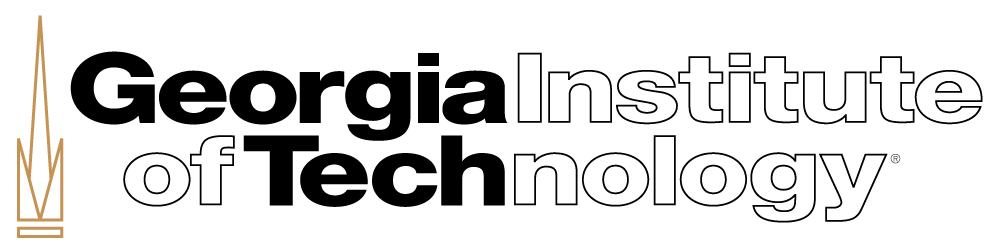
\includegraphics[scale=0.1]{figures/Gatech2.png}
 \hspace{155pt}
 
\includegraphics[scale=0.1]{figures/Gatech1.jpg}
 \titlepage
\end{frame}

%\maketitle

\begin{frame}{Background}
The goal of quantum chemistry is to solve the Schr{\"o}dinger equation for molecular systems
\begin{multicols}{2}
\begin{equation}
 -i \hbar \frac{\partial}{\partial t} \psi = \hat{H} \psi \nonumber
\end{equation}
\begin{figure}
 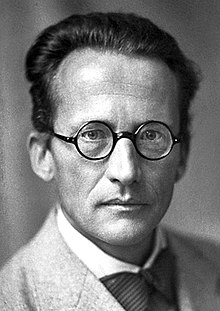
\includegraphics[scale=0.3]{figures/Schrodinger.jpg}\\
 E. Schr{\"o}dinger \\ (1887-1961)
\end{figure}
\end{multicols}
\end{frame}

\begin{frame}{Background}
Exact solution (within a finite basis) to the time-independent Schr{\"o}dinger equation is achieved by the {\it Full Configuration Interaction} (FCI) method:
\vspace{10pt}
\begin{enumerate}
 \item[1] Expand the wave function as
 \begin{equation}
  \Psi_{\rm FCI} = (\hat{1} + \hat{C}) \Phi_0,
 \end{equation}
  where $\Phi_0$ is a reference configuration (usually taken as the Hartree-Fock determinant), and 
  $\hat{C}$ is a linear excitation operator of the form
  \begin{equation}
   \hat{C} = \sum_{ia} c_i^a \hat{a}^\dagger_a \hat{a}_i + \frac{1}{4}\sum_{ijab} c_{ij}^{ab} \hat{a}^\dagger_a \hat{a}^\dagger_b \hat{a}_j \hat{a}_i + \cdots \,
  \end{equation}
  $i,j,k,\cdots \in \{\phi_{\rm occ.}\}$ and $a,b,c,\cdots \in \{\phi_{\rm virt.}\}$.
\end{enumerate}
\end{frame}

\begin{frame}{Background}
\onslide<1->{
Exact solution (within a finite basis) to the time-independent Schr{\"o}dinger equation is achieved by the {\it Full Configuration Interaction} (FCI) method:
\vspace{10pt}
\begin{enumerate}
  \item[2] Vocationally minimize the energy functional with respect to the $c$-coefficients 
  \begin{equation}
   \min_{\{c\}} E(\{c\}) = \frac{\langle \Phi_0 | (\hat{1} + \hat{C})^\dagger \hat{H} (\hat{1} + \hat{C})| \Phi_0 \rangle}{ \langle \Phi_0 | (\hat{1} + \hat{C})^\dagger (\hat{1} + \hat{C})| \Phi_0 \rangle
}  \end{equation}
}
\onslide<2->{
  which is equivalent to solve
  \begin{equation}
   \mathbf{E} = \mathbf{c}^\dagger \mathbf{H} \mathbf{c}
  \end{equation}
  aka, {\it full diagonalization}.
}
\end{enumerate}
\end{frame}

\begin{frame}{Background}
\onslide<1->{
 Problem with FCI for molecular systems:
}
 \vspace{10pt}
 \begin{itemize}
 \onslide<2->{
  \item The number of configurations in the FCI space grows combinatorially with respect to the system size
  \begin{equation}
   \dim \Psi_{\rm FCI} = \binom{K}{N},
  \end{equation}
  $K$ is the number of one-electron basis functions (spin orbitals) and $N$ is the number of electrons.\\
 }
  \vspace{10pt}
 \onslide<3->{
  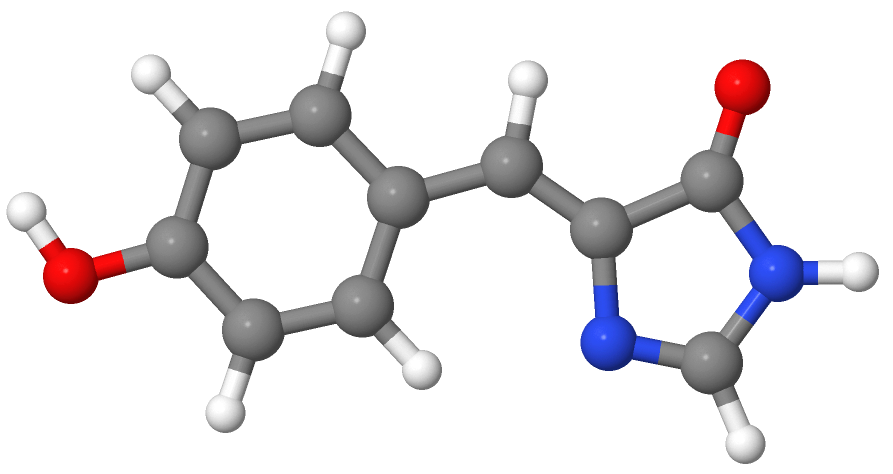
\includegraphics[scale=0.1]{figures/gfp.png}
  \textbf{GFP chromophore:} 1656 orbitals, 98 electrons, 10$^{314}$ configurations!
 }
 \end{itemize}
\end{frame}

\begin{frame}{Background}
\onslide<1->{
 Solution:
 \vspace{10pt}
 \begin{itemize}
  \item Truncate the FCI expansion at a given excitation level (usually after doubles excitations)
  \begin{equation}
   \hat{C} = \sum_{ia} c_i^a \hat{a}^\dagger_a \hat{a}_i + \frac{1}{4}\sum_{ijab} c_{ij}^{ab} \hat{a}^\dagger_a \hat{a}^\dagger_b \hat{a}_j \hat{a}_i.
  \end{equation}
}
\onslide<2->{
  Now, the number of configurations is only of the order $N^2 (K-N)^2$.\\
}
  \vspace{10pt}
\onslide<3->{
  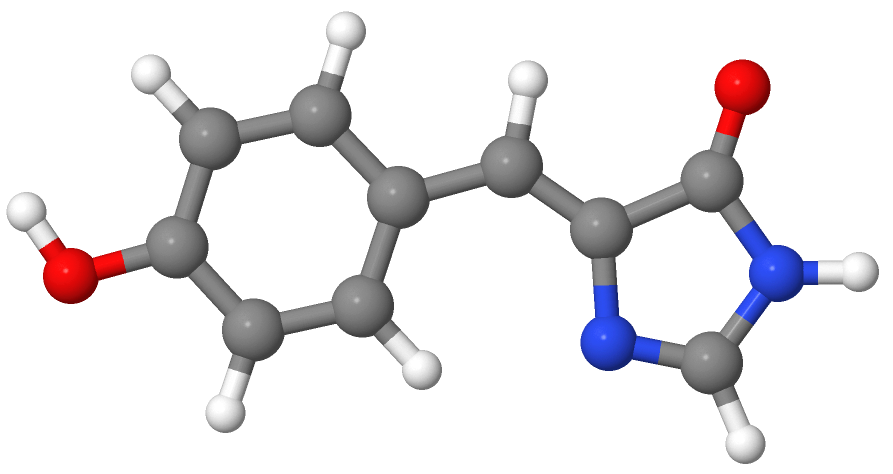
\includegraphics[scale=0.1]{figures/gfp.png}
  \textbf{GFP chromophore:} 1656 orbitals, 98 electrons, 10$^{10}$ configurations!
}
 \end{itemize}
\end{frame}

\begin{frame}{Background}
 Another problem emerges:
 \vspace{10pt}
 \begin{itemize}
  \item Truncated CI methods are not size-consistent \\
  \vspace{10pt}
  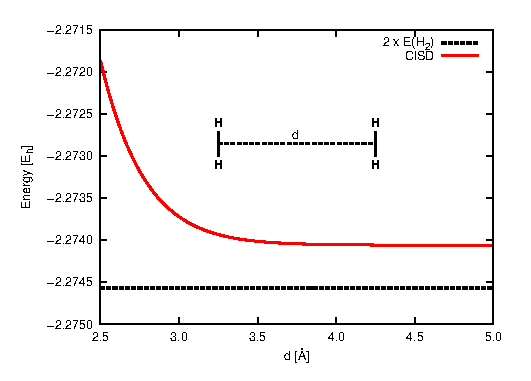
\includegraphics[scale=1.0]{figures/size_extensivity1.eps}
 \end{itemize}
\end{frame}

\begin{frame}{Background}
 Coupled-cluster theory comes to rescue...
  \begin{equation}
   \Psi_{\rm CC} = e^{\hat{T}} \Phi_0,
  \end{equation}
   where $\hat{T}$ is the cluster operator of the form
   \begin{equation}
    \hat{T} = \sum_{ia} t_i^a \hat{a}^\dagger_a \hat{a}_i + \frac{1}{4}\sum_{ijab} t_{ij}^{ab} \hat{a}^\dagger_a \hat{a}^\dagger_b \hat{a}_j \hat{a}_i + \cdots \,
   \end{equation}
   \begin{multicols}{2}
   \begin{figure}
   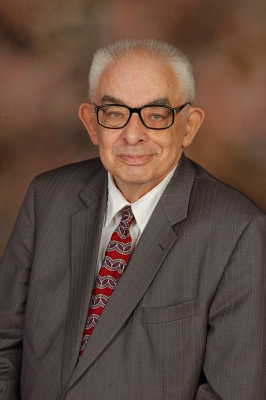
\includegraphics[scale=0.2]{figures/Cizek.jpg}\\
   J. {\v C}{\'i}{\v z}ek
   \end{figure}

   \begin{figure}
   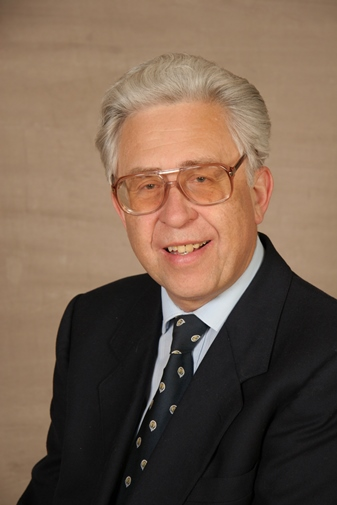
\includegraphics[scale=0.33]{figures/Paldus.jpg}\\
   J. Paldus
   \end{figure}
   \end{multicols}
\end{frame}

\begin{frame}{Background}
 Coupled-cluster theory comes to rescue...
 \vspace{10pt}
 \begin{itemize}
  \item Truncated CC methods {\bf are} size-consistent \\
  \vspace{10pt}
  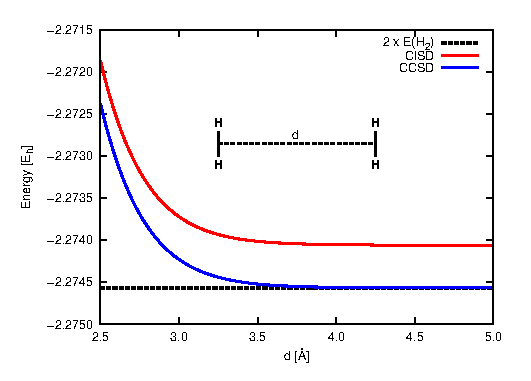
\includegraphics[scale=1.0]{figures/size_extensivity.eps}
 \end{itemize}
\end{frame}

\begin{frame}{CC theory for ground states}
 \onslide<1-4>{Projective approach for solving the CC equation
  \begin{equation}
   \hat{H} e^{\hat{T}} |\Phi_0 \rangle = E_{\rm CC} e^{\hat{T}} |\Phi_0 \rangle
  \end{equation}
 }
 \onslide<2-4>{left multiply both sides by $e^{-\hat{T}}$
  \begin{equation}
   e^{-\hat{T}} \hat{H} e^{\hat{T}} |\Phi_0 \rangle = E_{\rm CC}  |\Phi_0 \rangle.
  \end{equation}
 } 
 \onslide<3-4>{The energy is then computed by solving  
  \begin{equation}
   \langle \Phi_0 | e^{-\hat{T}} \hat{H} e^{\hat{T}} |\Phi_0 \rangle = E_{\rm CC},
  \end{equation}
 }
 \onslide<4>{and the $t$-amplitudes by
  \begin{equation}
   \langle \Phi_{ijk\cdots}^{abc\cdots} | e^{-\hat{T}} \hat{H} e^{\hat{T}} |\Phi_0 \rangle = 0 ~ \forall~ t_i^a, t_{ij}^{ab}, \cdots.
  \end{equation}
 }
\end{frame}

\begin{frame}{CC theory for ground states}
 \onslide<1->{Properties of CC Hamiltonian and Energy}
 \begin{itemize}
  \onslide<2->{\item The projective approach yields non-variational energies!}
  \onslide<3->{\item The CC effective Hamiltonian $\bar{H}$ is computed by similarity-transforming the electronic Hamiltonian $\hat{H}$,
  \begin{eqnarray}
   \bar{H} &=& e^{-\hat{T}} \hat{H} e^{\hat{T}} \\ \nonumber
           &=& \hat{H} + [\hat{H},\hat{T}] + \frac{1}{2} [[\hat{H},\hat{T}],\hat{T}] \\ \nonumber 
           &+& \frac{1}{6} [[[\hat{H},\hat{T}],\hat{T}],\hat{T}] + \frac{1}{24}[[[[\hat{H},\hat{T}],\hat{T}],\hat{T}] ,\hat{T}]
  \end{eqnarray}
  }
  \onslide<4->{Thus, $\bar{H}$ is non-symmetric and $\langle \Psi_{\rm CC}| \neq (|\Psi_{\rm CC}\rangle)^\dagger$.}
 \end{itemize}
\end{frame}


\begin{frame}{CC theory for excited state properties}
 \onslide<1->{The equation-of-motion (EOM) formalism}
 \onslide<2->{
  \begin{eqnarray}
   |\Psi_m \rangle &=& \sum_{I = 0}^{M} \hat{R}_I^m e^{\hat{T}} |\Phi_0 \rangle \\
   \langle \tilde{\Psi}_m |&=& \sum_{I = 0}^{M} \langle \Phi_0| e^{-\hat{T}} \hat{L}_I^m 
  \end{eqnarray}
  Here, $\hat{R}$ ($\hat{L}$) is a linear excitation (de-excitation) operator for the $m$-th excited state including up to $M$-electrons excitations.\
 }
 \vspace{10pt}
 \onslide<3->{
  Excitation energies and excited-state wave functions are obtained as
  \begin{eqnarray}
   (\bar{H} - E_{\rm CC}) |\Psi_m \rangle &=& \omega_m |\Psi_m \rangle \\
   \langle \tilde{\Psi}_m | (\bar{H} - E_{\rm CC}) &=& \langle \tilde{\Psi}_m | \omega_m
  \end{eqnarray}
 }
 \onslide<4->{
  \color{red}{Diagonalize $\mathbf{\tilde{H}} = \mathbf{\bar{H}} - \mathbf{E_{\rm CC}}$?}
 }
\end{frame}

\begin{frame}{CC theory for excited state properties}
 \onslide<1->{
 A simple illustration...\\
 }
 \vspace{10pt}
 \onslide<2->{
 Let's consider the carbon monoxide molecule in an augmented triple-$\zeta$ basis (14 electrons in 92 orbitals):
 }
 \onslide<3->{
  \begin{equation}
   \dim \Psi_{\rm EOM-CCSD} \approx \mathcal{O}(N^2 [K-N]^2)
  \end{equation}
 }
 \onslide<4->{
  \begin{equation}
   \dim \Psi_{\rm EOM-CCSD} \approx 10^5
  \end{equation}
 }
 \onslide<5->{
 Thus, $\dim \mathbf{\tilde{H}} \approx 10^5 \times 10^5$.\\
 }
 \vspace{10pt}
 \onslide<6->{
 Memory requirement: {\bf $>$700 GB} just to store $\mathbf{\tilde{H}}$.\\
 }
 \vspace{10pt}
 \onslide<7->{
 This bottleneck is usually bypassed by the use of partial diagonalization algorithms.
 }
\end{frame}

\begin{frame}{CC theory for excited state properties}
\onslide<1->{
 But sometimes, partial diagonalization is not sufficient!\\
 \vspace{10pt}
 \begin{center}
 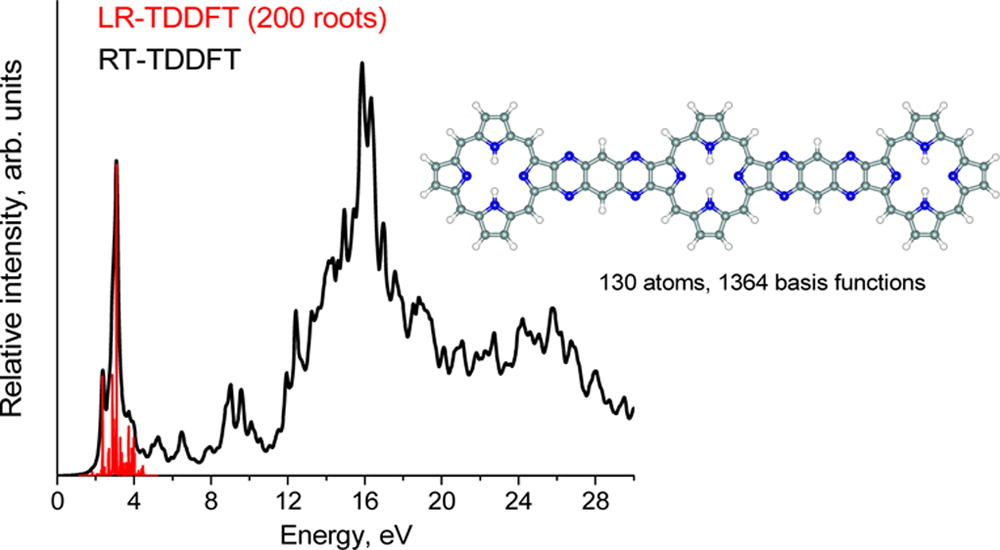
\includegraphics[scale=1]{figures/big_molecule.jpeg}
 \end{center}
}
\onslide<2->{
 200 roots does not contain enough information \footnote{S. Tussupbayev et al. JCTC, 11, 1102 (2015)}.\\
}
 \vspace{10pt}
 \onslide<3->{
 \color{red}{The solution is the explicit time propagation!}
}
\end{frame}

\begin{frame}{Time-domain CC theory for linear absorption spectra}
 \onslide<1->{
 From linear response theory,
 \begin{equation}
  I(\omega) =  \sum_{m} \langle \tilde{\Psi}_0 | \bar{\mu}| \Psi_m \rangle \langle \tilde{ \Psi}_m| \bar{\mu}| \Psi_0 \rangle \delta(\omega_m - \omega).
 \end{equation}
 }
 \onslide<2->{
 By using
 \begin{equation}
  \delta(\omega_m - \omega) = \int_{- \infty}^{\infty}  dt~ e^{i(\omega_{m} - \omega)t} \nonumber ,
 \end{equation}
 }
 \onslide<3->{
 we end up with
 \begin{equation}
 I(\omega) =  \int_{-\infty}^{\infty}  dt~ e^{-i \omega t}\underbrace{ \langle \tilde{ \Psi}_0 | \bar{\mu} }_{\langle \tilde{M}_0|} e^{i\tilde{H}t}\underbrace{\bar{\mu}| \Psi_0 \rangle}_{|M_0\rangle}
 \end{equation}
 }
 \onslide<4->{
 which can finally be rewritten as
 \begin{block}{}
  \begin{equation}
  \color{blue}{I(\omega) =  \int_{-\infty}^{\infty}  dt~ e^{-i \omega t}{\langle \tilde{M}(0)|M(-t)\rangle}} 
  \end{equation}
 \end{block}
 }
\end{frame}

\begin{frame}{Time-domain CC theory for linear absorption spectra}
 For more details...\\
 \vspace{10pt}
 \begin{center}
 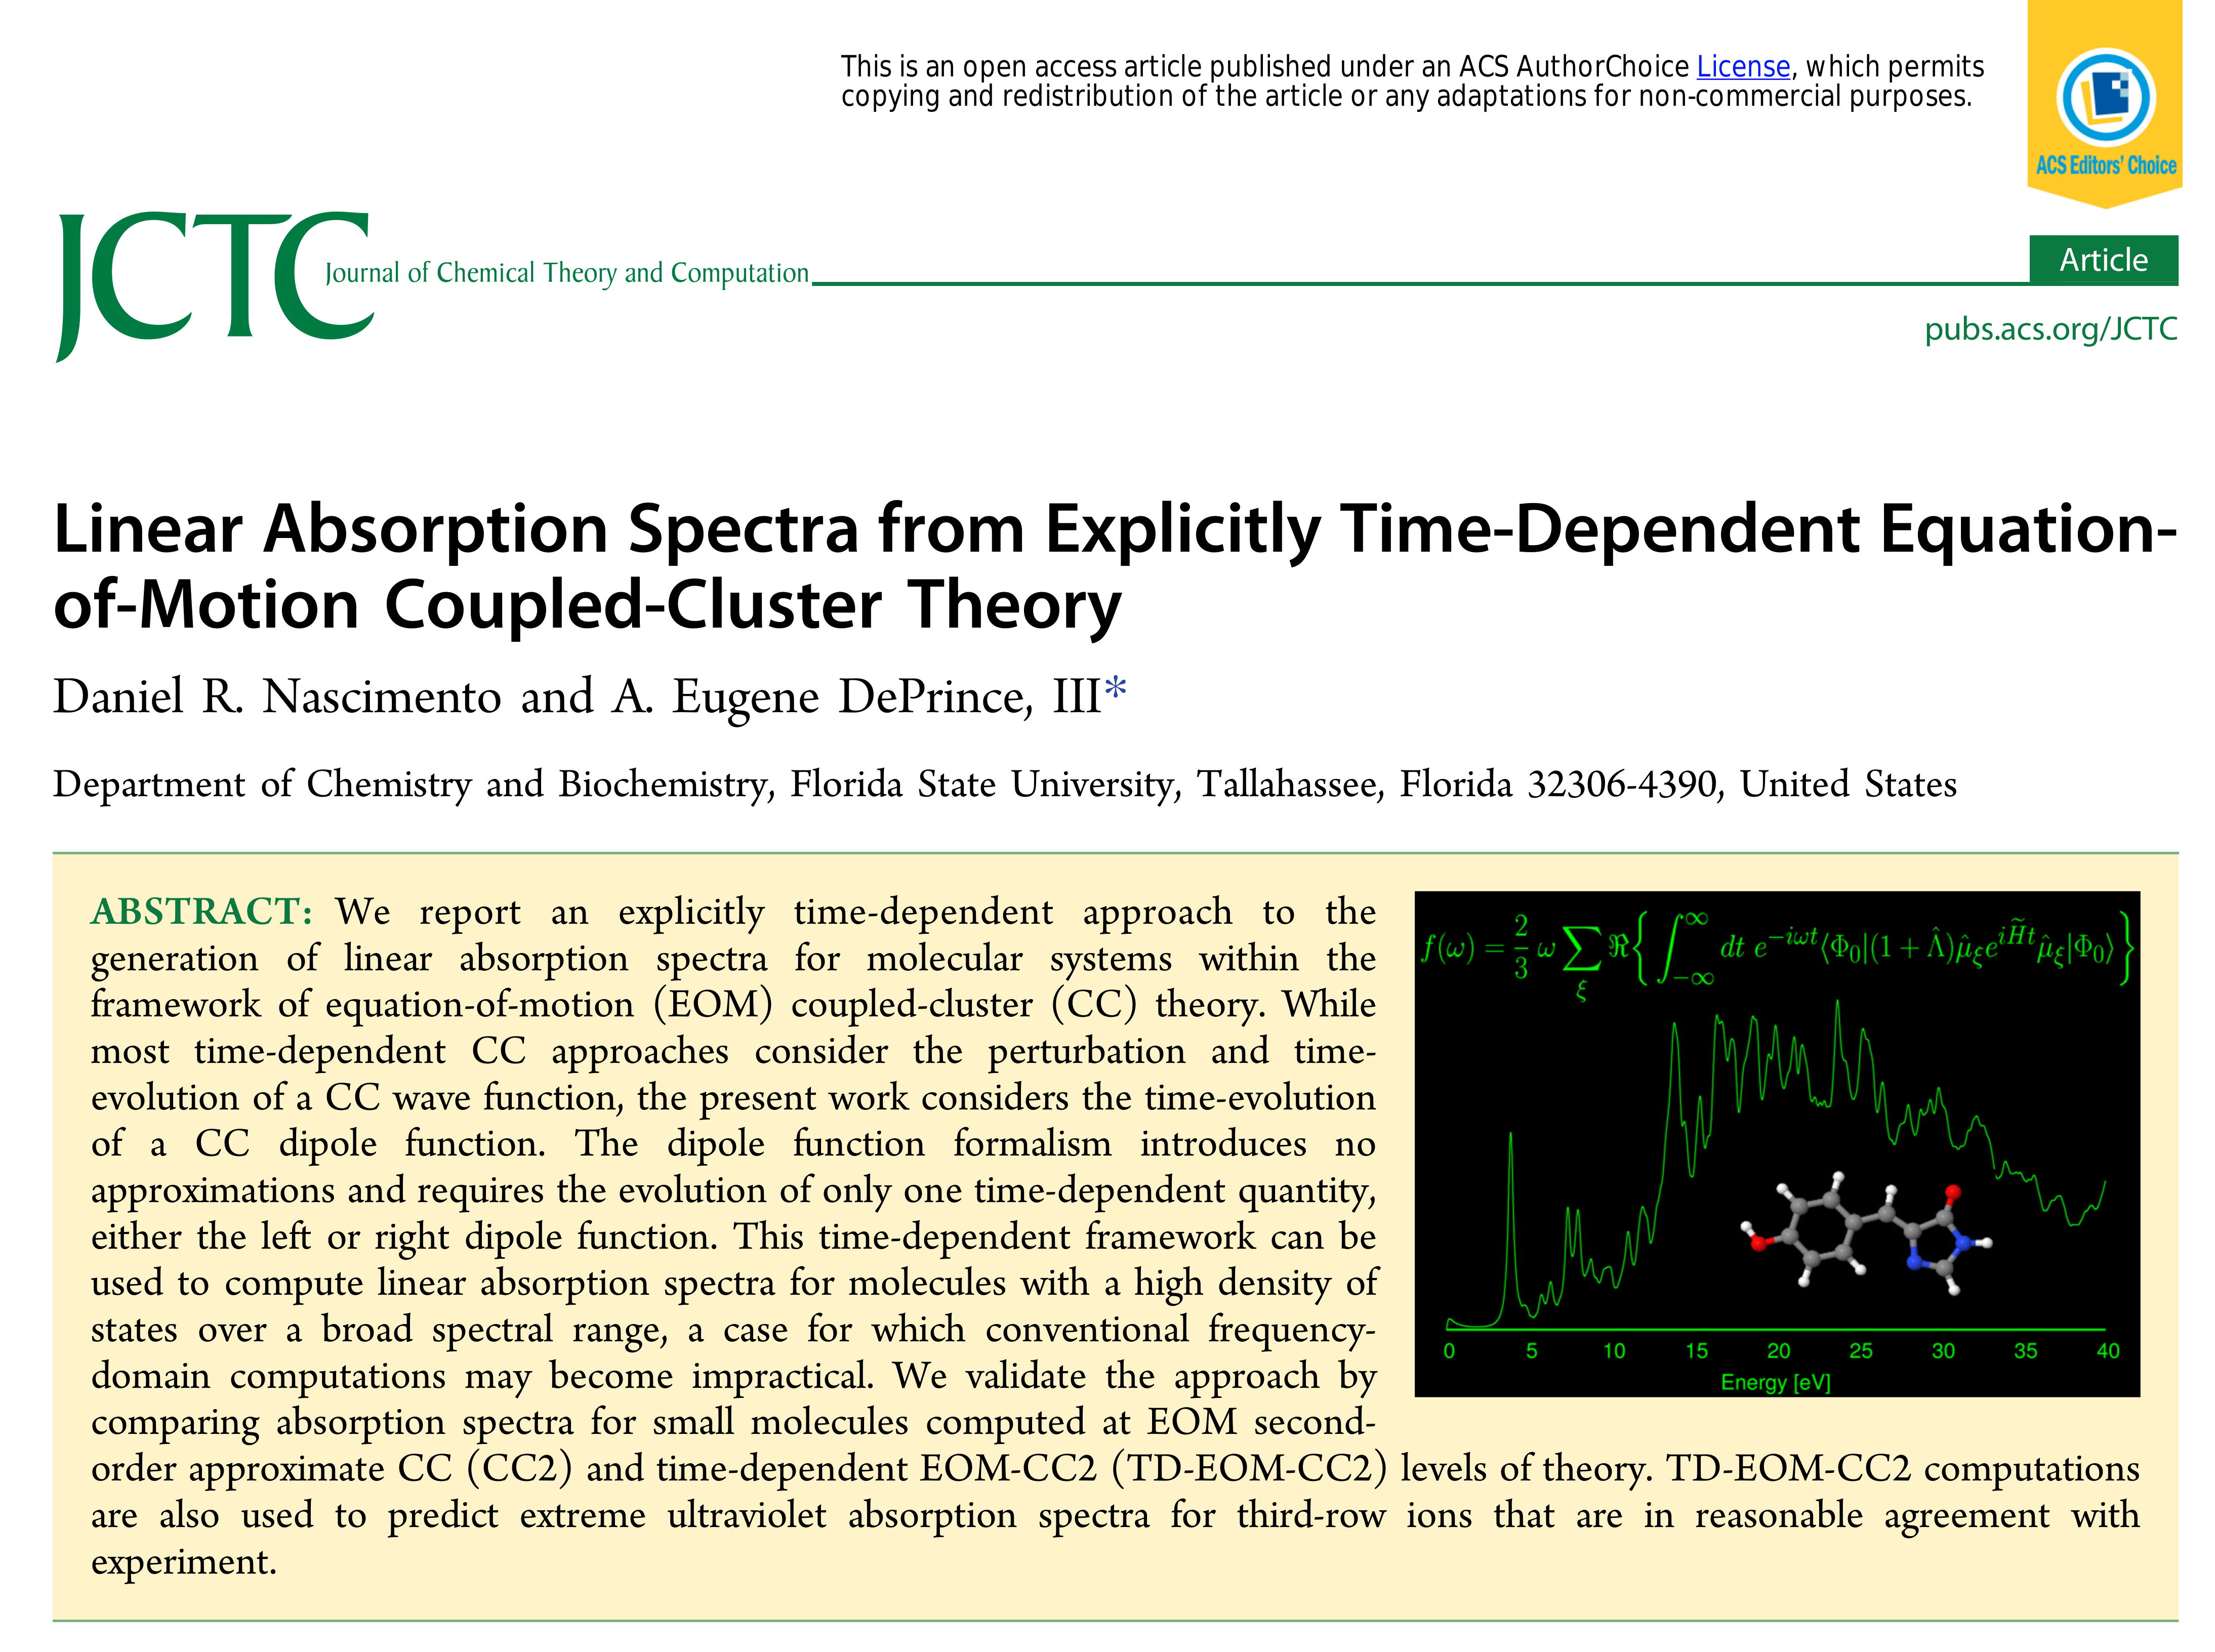
\includegraphics[scale=0.5]{figures/jctc.png} 
 \end{center}
\end{frame}

\begin{frame}{Time-domain CC theory for linear absorption spectra}
 TD-EOM-CC2 vs EOM-CC2

 \begin{center}
 \begin{tikzpicture}
            \node[anchor=south west,inner sep=0] (image) at (0,0) {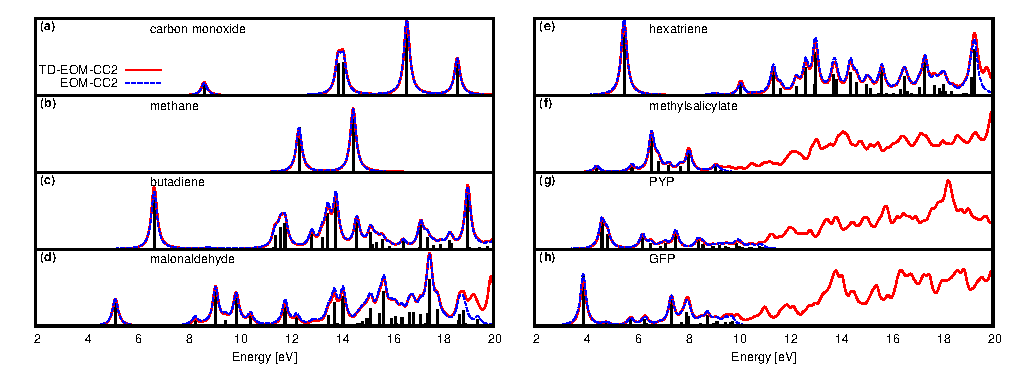
\includegraphics[scale=1.0,trim={0 0 3.33in 0},clip]{figures/left_v2.eps}};
            \node[align=center,blue,font={\small}] at (1.3in,2.1in) {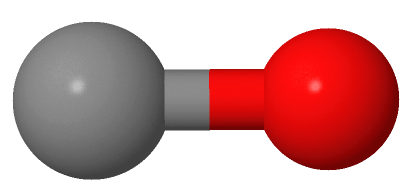
\includegraphics[scale=0.05]{figures/co.png}};
            \node[align=center,blue,font={\small}] at (1.3in,1.5in) {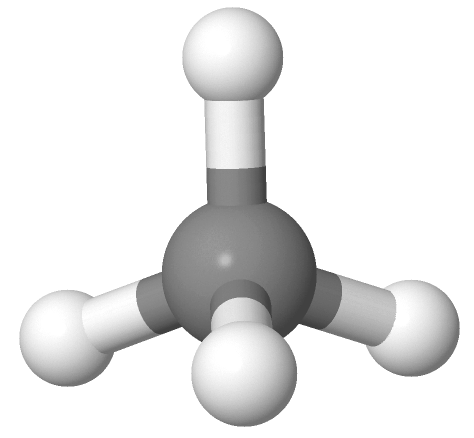
\includegraphics[scale=0.05]{figures/methane.png}};
            \node[align=center,blue,font={\small}] at (1.3in,1.0in) {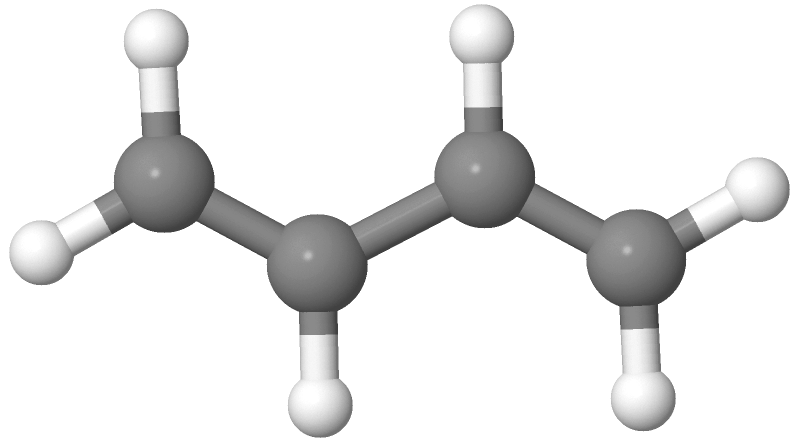
\includegraphics[scale=0.05]{figures/butadiene.png}};
            \node[align=center,blue,font={\small}] at (0.95in,0.5in) {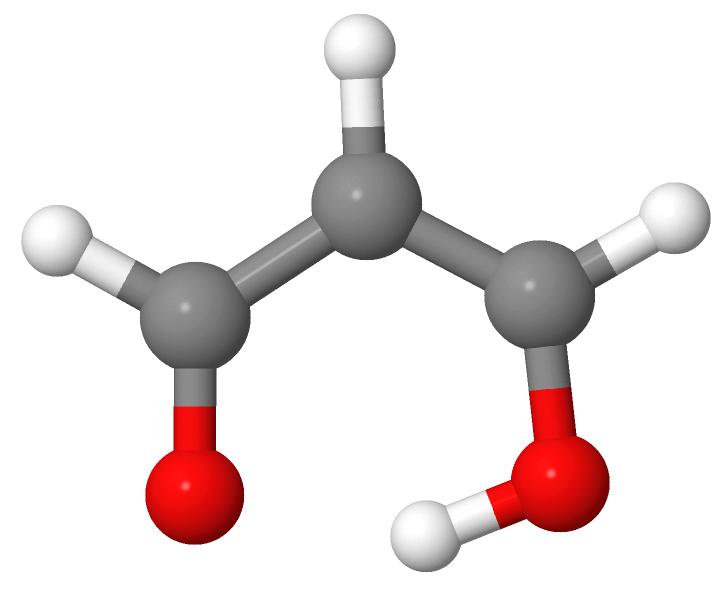
\includegraphics[scale=0.04]{figures/malonaldehyde.png}};

 \end{tikzpicture}
 \end{center}
  \footnotesize{D. R. Nascimento and A. E. DePrince, {\it JCTC}, {\bf 12}, 5834, (2016) }
\end{frame}

\begin{frame}{Time-domain CC theory for linear absorption spectra}
 TD-EOM-CC2 vs EOM-CC2

 \begin{center}
 \begin{tikzpicture}
            \node[anchor=south west,inner sep=0] (image) at (0,0) {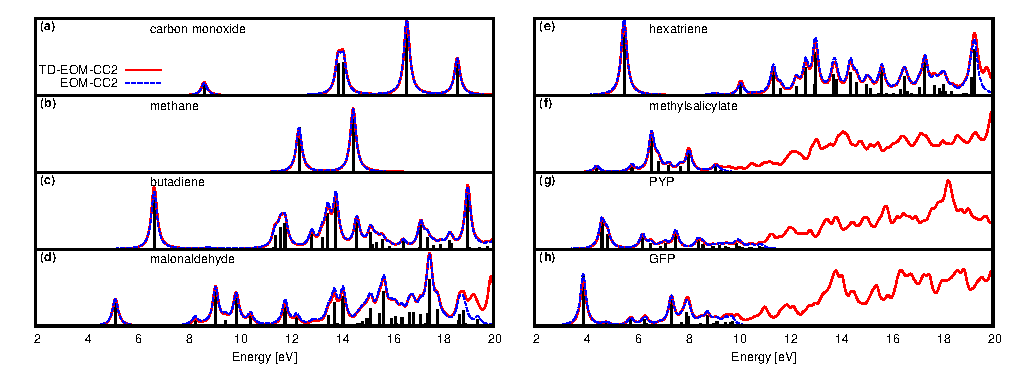
\includegraphics[scale=1.0,trim={3.33in 0 0 0},clip]{figures/left_v2.eps}};
            \node[align=center,blue,font={\small}] at (-0.5in,0.5in) {50 roots};
            \node[align=center,blue,font={\small}] at (-0.5in,1.0in) {50 roots};
            \node[align=center,blue,font={\small}] at (-0.5in,1.5in) {20 roots};
            \node[align=center,blue,font={\small}] at (-0.5in,2.0in) {100 roots};
            \node[align=center,blue,font={\small}] at (1.1in,2.0in) {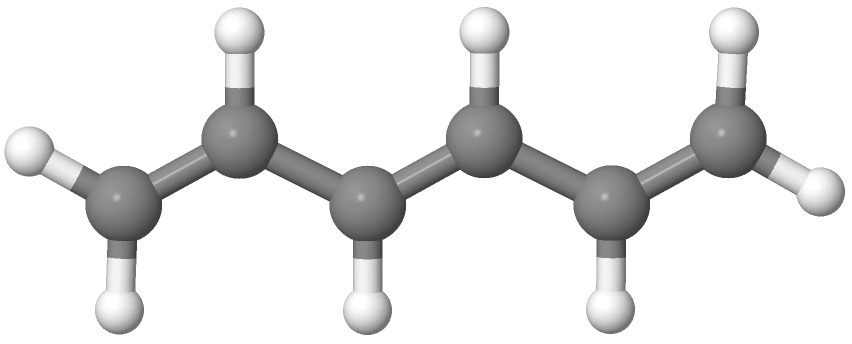
\includegraphics[scale=0.05]{figures/hexatriene.png}};
            \node[align=center,blue,font={\small}] at (0.5in,1.54in) {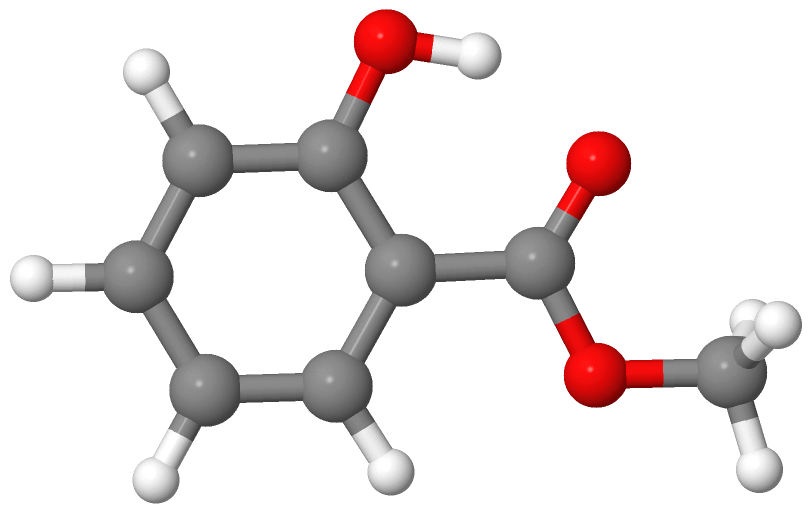
\includegraphics[scale=0.045]{figures/methylsalycilate.png}};
            \node[align=center,blue,font={\small}] at (1.3in,1.05in) {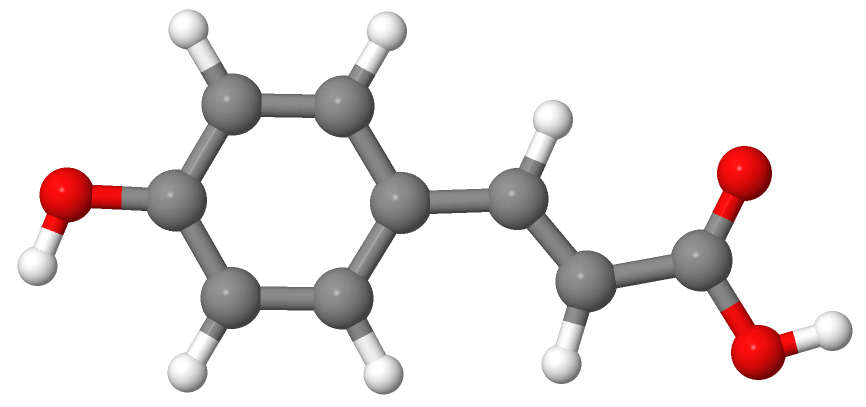
\includegraphics[scale=0.05]{figures/pyp.png}};
            \node[align=center,blue,font={\small}] at (0.75in,0.5in) {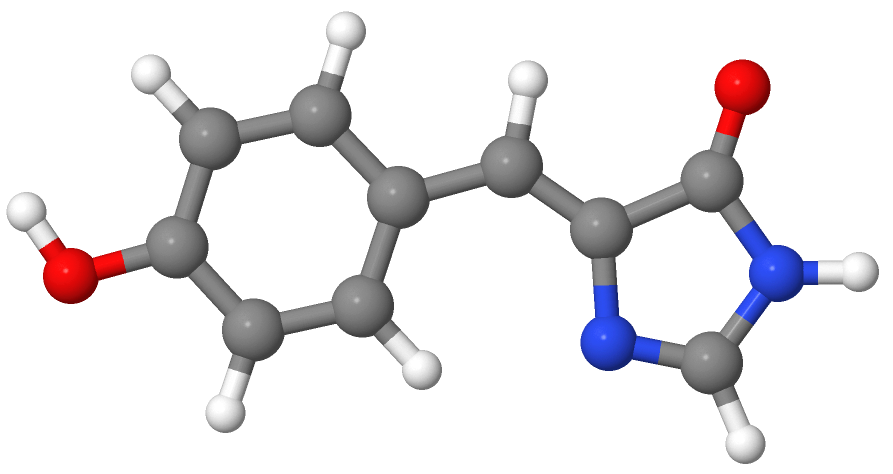
\includegraphics[scale=0.04]{figures/gfp.png}};
 \end{tikzpicture}
 \end{center}
 \footnotesize{D. R. Nascimento and A. E. DePrince, {\it JCTC}, {\bf 12}, 5834, (2016) }
\end{frame}

\begin{frame}{Time-domain CC theory for linear absorption spectra}
 Extreme UV spectrum of the Neon isoelectronic series

 \begin{center}
   \begin{tikzpicture}
            \node[anchor=south west,inner sep=0] (image) at (0,0) {\includegraphics[scale=1.0,trim={0 2.4in 3.45in 0},clip]{figures/d2.eps}};
            \node[align=center,blue,font={\small}] at (1.8in,1.5in) {Na$^+$};
  \end{tikzpicture} 
 \end{center}
 \footnotesize{D. R. Nascimento and A. E. DePrince, {\it JCTC}, {\bf 12}, 5834, (2016) }\\
 \footnotesize{A. Gray, Ph.D. thesis, Dublin City University (1999)} 
\end{frame}

\begin{frame}{Time-domain CC theory for linear absorption spectra}
 Extreme UV spectrum of the Neon isoelectronic series

 \begin{center}
  \begin{tikzpicture}
            \node[anchor=south west,inner sep=0] (image) at (0,0) {\includegraphics[scale=0.5]{figures/d2.eps}};
            \node[align=center,blue,font={\small}] at (0.9in,2.0in) {Na$^+$};
            \node[align=center,blue,font={\small}] at (2.7in,2.0in) {Mg$^{2+}$};
            \node[align=center,blue,font={\small}] at (0.9in,0.8in) {Al$^{3+}$};
            \node[align=center,blue,font={\small}] at (2.9in,0.8in) {Si$^{4+}$};
  \end{tikzpicture} 
 \end{center}
 \footnotesize{D. R. Nascimento and A. E. DePrince, {\it JCTC}, {\bf 12}, 5834, (2016) }\\
 \footnotesize{A. Gray, Ph.D. thesis, Dublin City University (1999)} 
\end{frame}

\begin{frame}{Time-domain CC theory for linear absorption spectra}
 \begin{itemize}
 \onslide<1->{
  \item Prototype code available for \small{Psi4Numpy}
  \begin{center}
  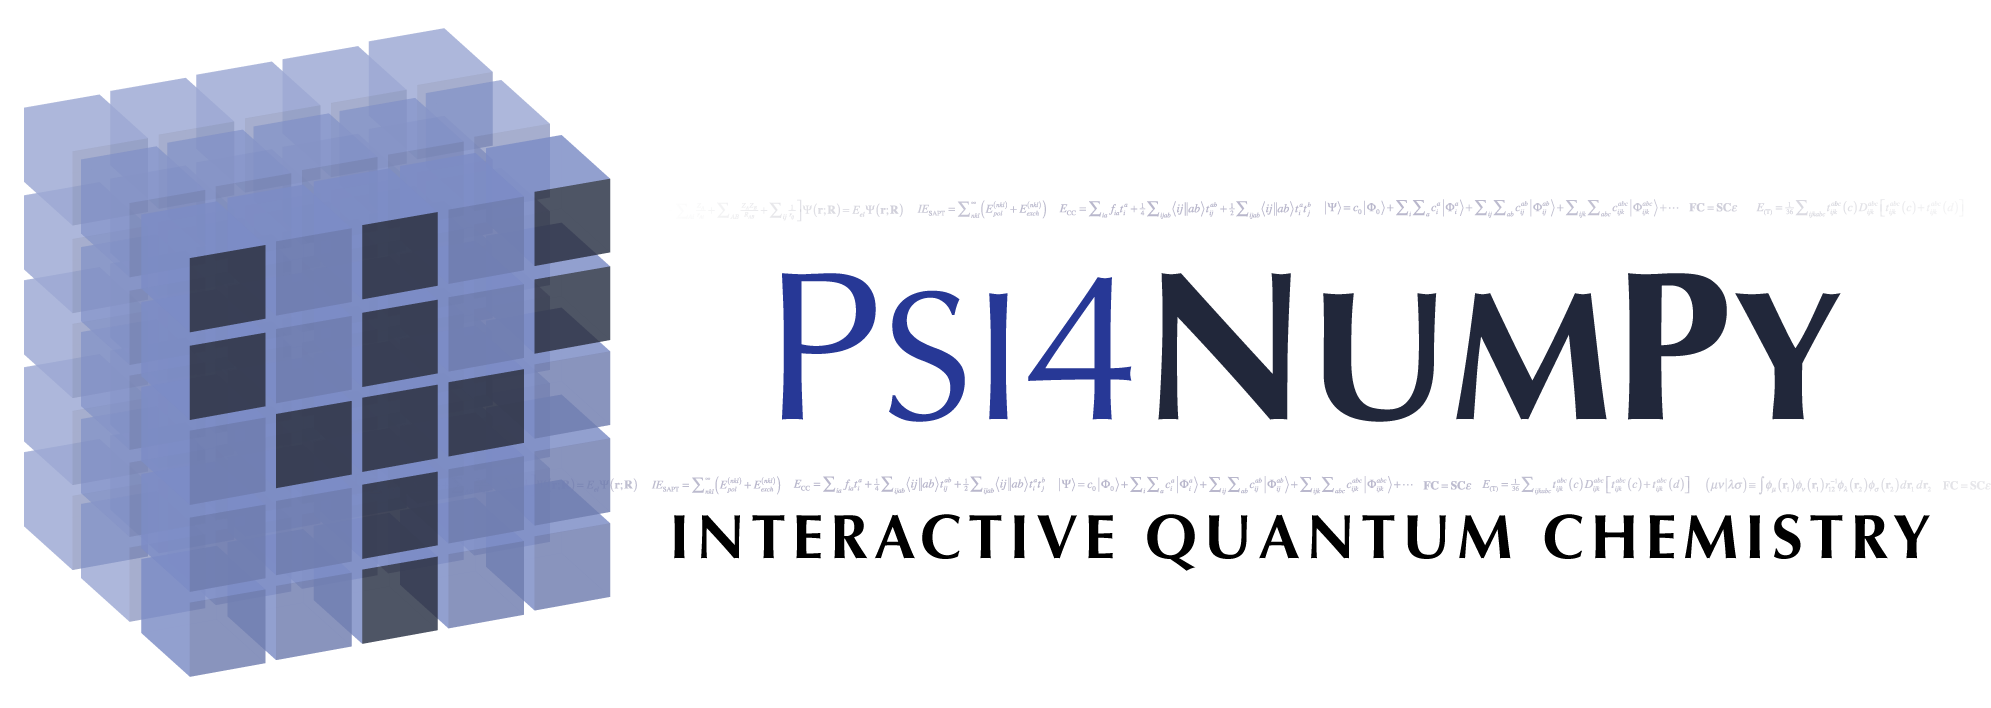
\includegraphics[scale=0.4]{figures/psi4numpybanner.png}
  \end{center}
 }
 \onslide<2->{
  \item Production level code will be released on \small{Chronus Quantum}
  \begin{center}
  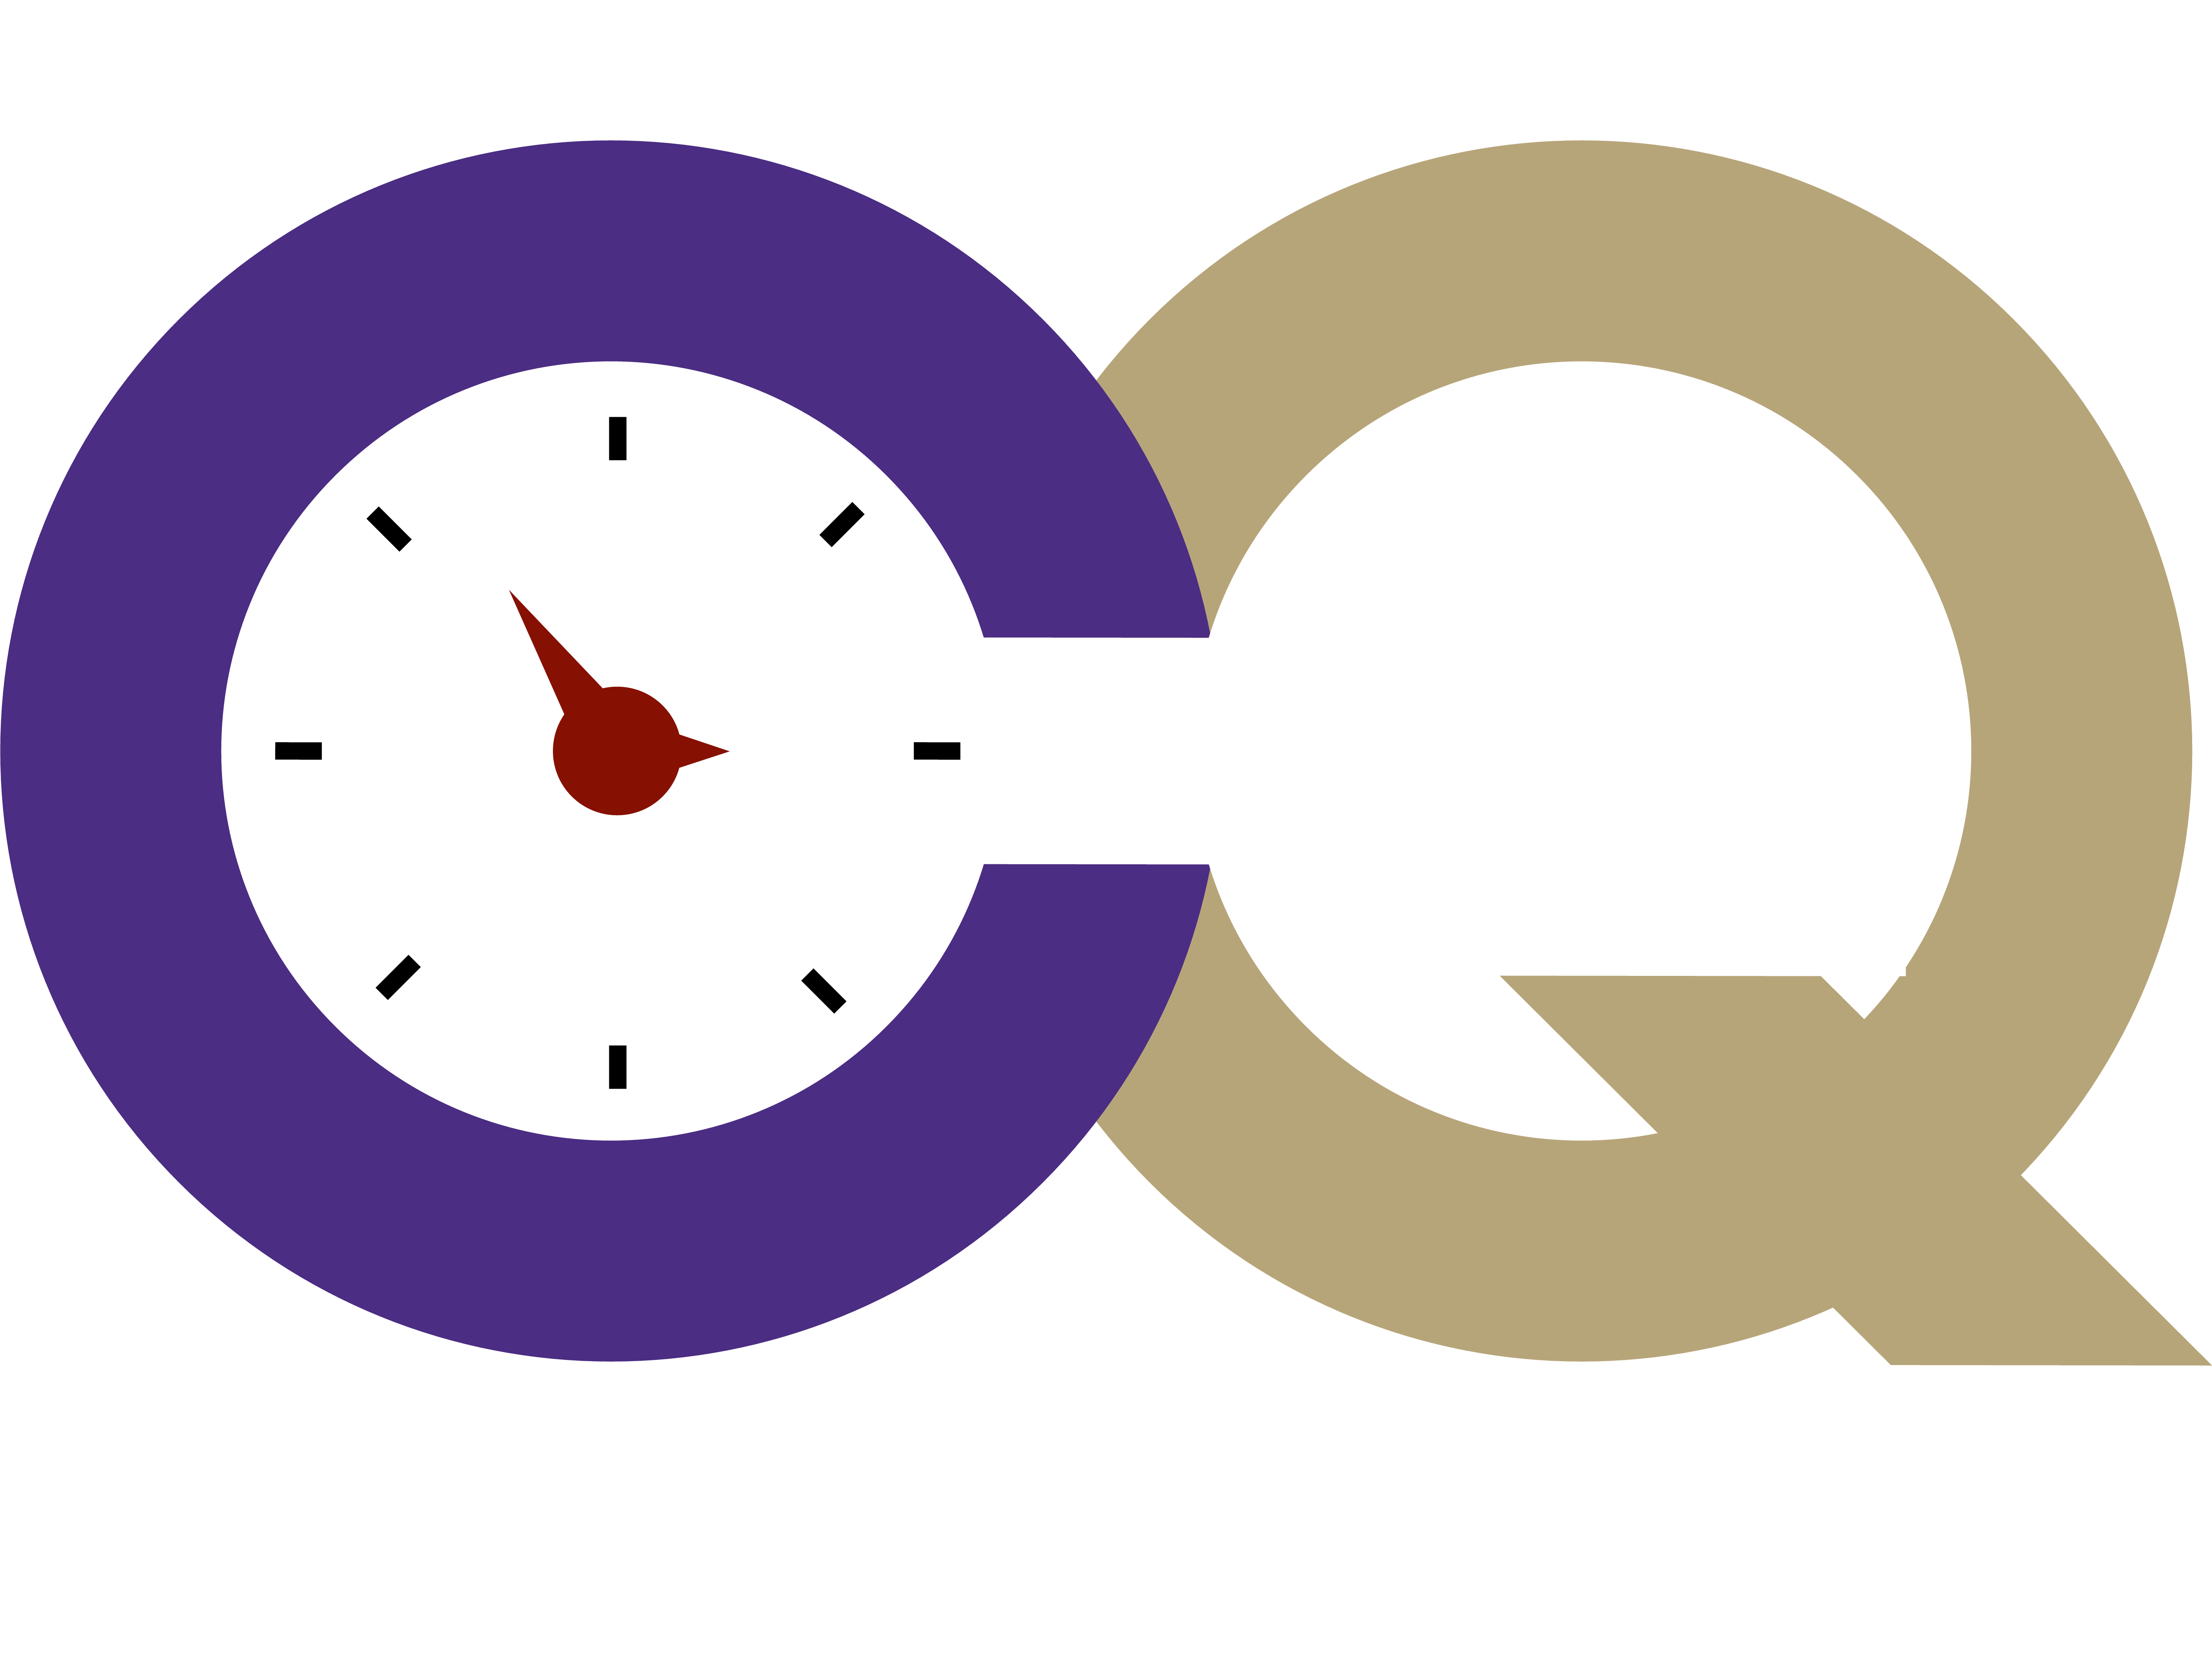
\includegraphics[scale=0.02]{figures/cq_logo.png}
  \end{center}
 }
\end{itemize}
\onslide<3->{
 \footnotesize{github.com/psi4/psi4numpy}, 
 \footnotesize{D. G. A. Smith {\it et al.}, {\it JCTC}, Article ASAP}
 \footnotesize{github.com/liresearchgroup/chronusq\_public}
}
\end{frame}

\begin{frame}{Caveats of TD-CC methods}
Simulations are subject to the Nyquist criteria
\begin{multicols}{2}
\begin{equation}
 \max \{\omega\} \le \frac{1}{2} \Gamma_{\rm sampling} \nonumber
\end{equation}
\begin{figure}
 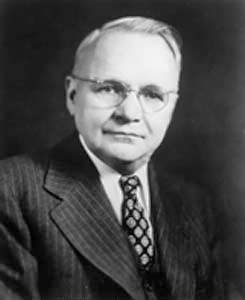
\includegraphics[scale=0.4]{figures/Harry_Nyquist.jpg}\\
 Harry Nyquist \\ (1889-1976)
\end{figure}
\end{multicols}
\end{frame}

\begin{frame}{Caveats of TD-CC methods}
Simulations are subject to the Nyquist criteria
\begin{center}
  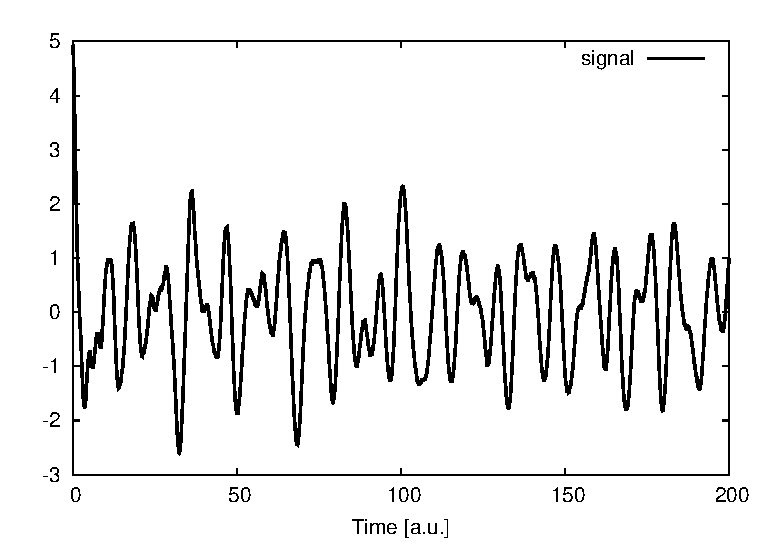
\includegraphics[scale=0.8]{figures/nyquist1.eps}
\end{center}
\end{frame}

\begin{frame}{Caveats of TD-CC methods}
Simulations are subject to the Nyquist criteria
\begin{center}
  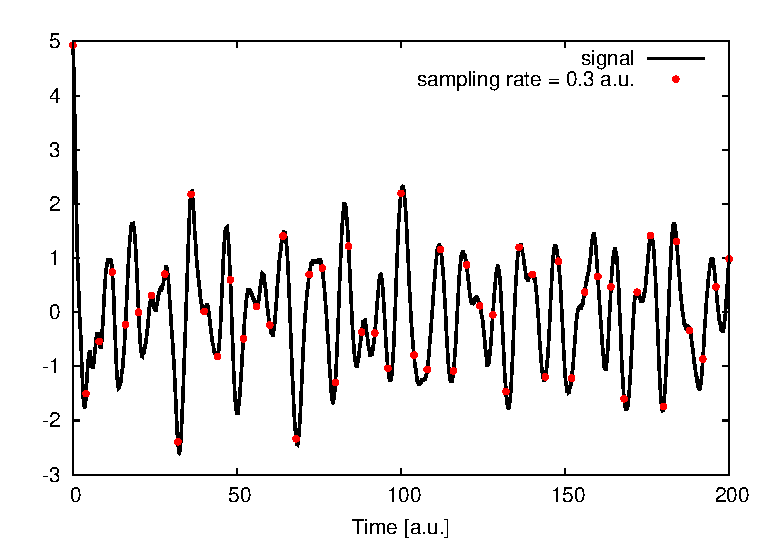
\includegraphics[scale=0.8]{figures/nyquist2.eps}
\end{center}
\end{frame}

\begin{frame}{Caveats of TD-CC methods}
Simulations are subject to the Nyquist criteria
\begin{center}
  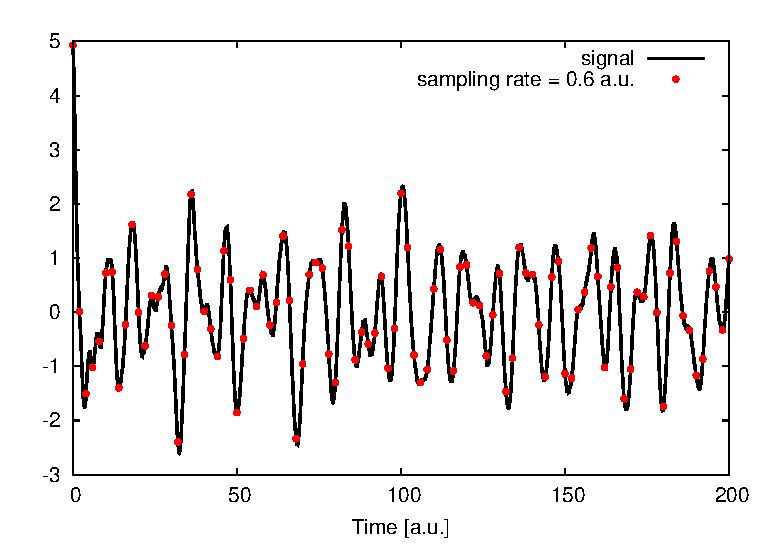
\includegraphics[scale=0.8]{figures/nyquist3.eps}
\end{center}
\end{frame}

\begin{frame}{Caveats of TD-CC methods}
Simulations are subject to the Nyquist criteria
\begin{center}
  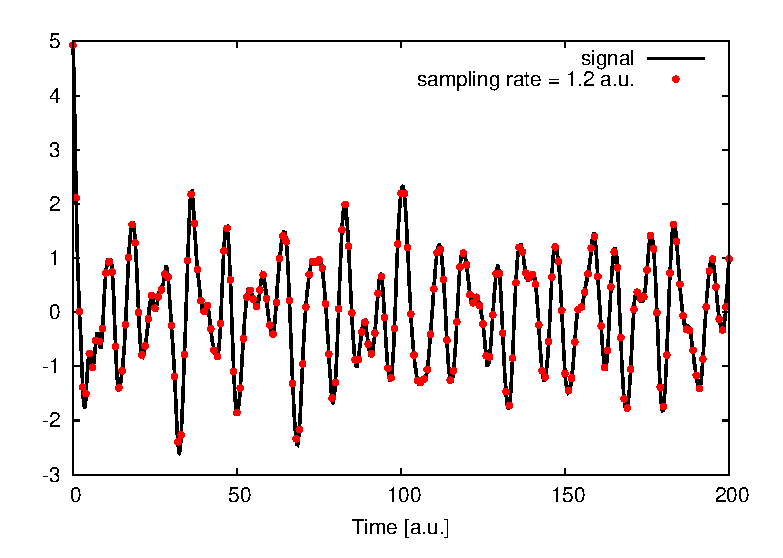
\includegraphics[scale=0.8]{figures/nyquist4.eps}
\end{center}
\end{frame}

\begin{frame}{Caveats of TD-CC methods}
Simulations are subject to the Nyquist criteria
\begin{center}
  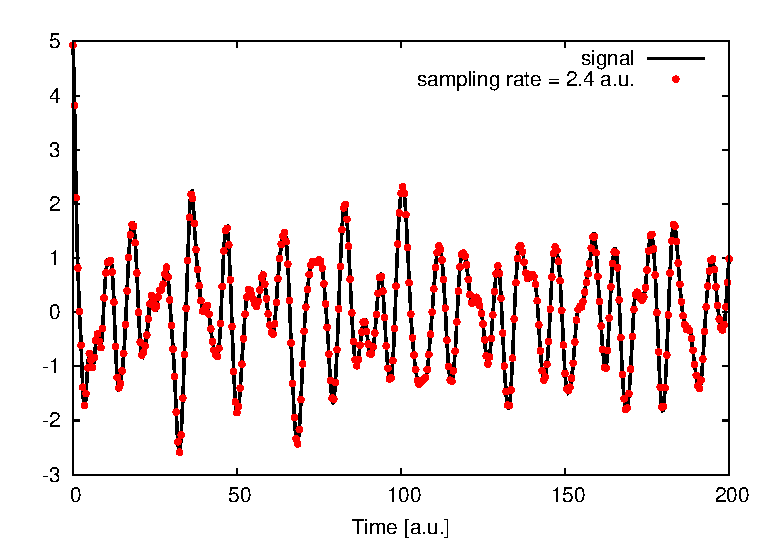
\includegraphics[scale=0.8]{figures/nyquist5.eps}
\end{center}
\end{frame}

\begin{frame}{Caveats of TD-CC methods}
Simulations are subject to the Nyquist criteria
\begin{center}
 \begin{tikzpicture}
 \onslide<1->{
            \node[anchor=south west,inner sep=0] (image) at (0,0) {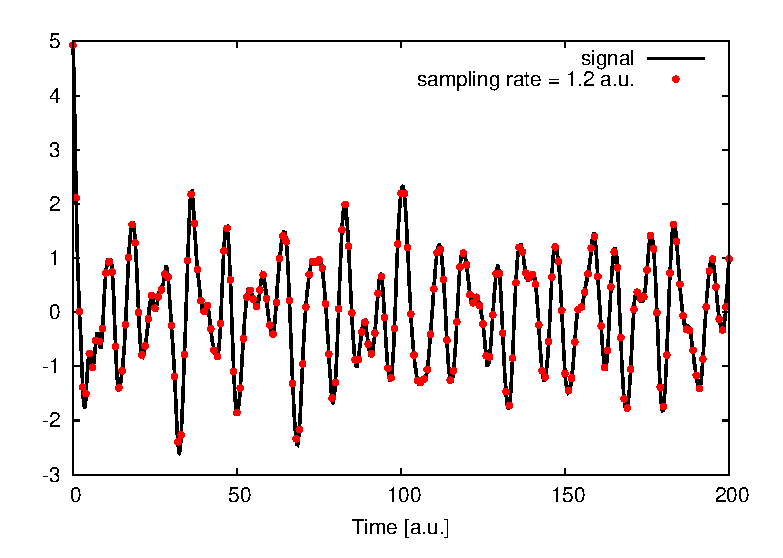
\includegraphics[scale=0.8]{figures/nyquist4.eps}};
 }
 \onslide<2->{
            \node[align=center,draw,line width=2pt,blue,font={\Huge},circle] at (0.88in,0.52in) {.};
            \node[align=center,draw,line width=2pt,blue,font={\Huge},circle] at (2.05in,1.9in) {.};
 }
 \onslide<3->{
            \node[align=center,blue,font={\small}] at (1.4in,2.2in) {Higher sampling rates are required to \\ fully recover the oscillator strength!};
 }
  \end{tikzpicture} 
\end{center}
\end{frame}

\begin{frame}{Accelerating convergence using Pad{\'e} approximants}
\onslide<1->{
Back to the line shape function...
 \begin{equation}
 I(\omega) =  \int_{-\infty}^{\infty}  dt~ e^{i \omega t} \langle  \tilde{M}(0)|M(t)\rangle   \nonumber
\end{equation}
}
\begin{multicols}{2}
\onslide<2->{
Change of variables such that
\begin{eqnarray}
 c_k &\equiv& \langle  \tilde{M}(0)|M(k\Delta t)\rangle \nonumber \\
 z_k &\equiv& e^{i \omega \Delta t} \nonumber
\end{eqnarray}
}
\vspace{-25pt}
\onslide<3->{
\begin{eqnarray}
\onslide<3->{
 I(z) &=& \sum_{k=0}^K c_k (z_k)^k \nonumber \\
}
\onslide<4->{ 
 \sum_{k=0}^K c_k (z_k)^k &=& \frac{\sum_{k=0}^{K/2} a_k  (z_k)^k}{\sum_{k=0}^{K/2} b_k (z_k)^k} \nonumber
} 
\end{eqnarray}
}
\onslide<4->{
\begin{figure}
 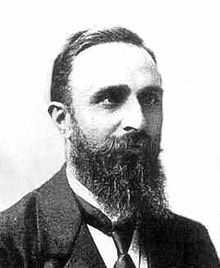
\includegraphics[scale=0.3]{figures/Pade.jpeg}\\
 Henry Pad{\'e} \\ (1863-1953)
\end{figure}
}
\end{multicols}
\onslide<5->{
\footnotesize{A. Bruner, D. LaMaster, and K. Lopata, {\it JCTC}, {\bf 12}, 3741 (2016)}
}
\end{frame}

\begin{frame}{Accelerating convergence using Pad{\'e} approximants}
Convergence @ C K-edge of carbon monoxide
\begin{center}
 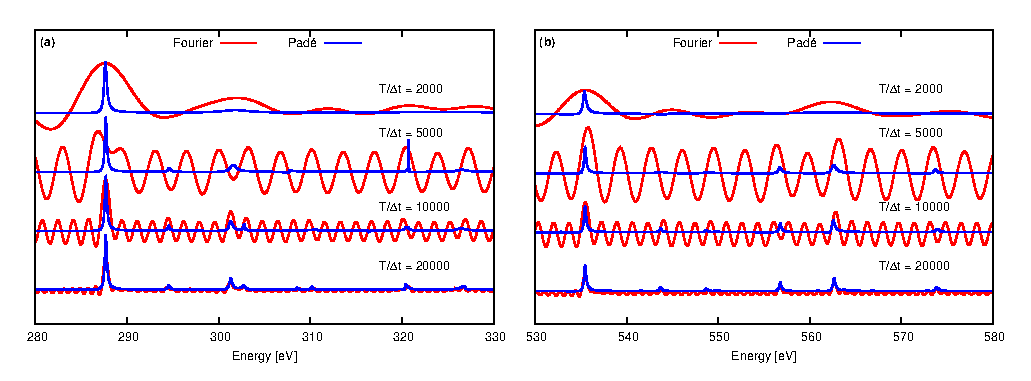
\includegraphics[scale=1.0,trim={0 0 3.33in 0},clip]{figures/convergence.eps}\\
\end{center}
\footnotesize{D. R. Nascimento and A. E. DePrince, {\it JPCL}, {\bf 8}, 2951, (2017)} 
\end{frame}

\begin{frame}{Accelerating convergence using Pad{\'e} approximants}
Broadband linear absorption spectrum of carbon monoxide
\begin{center}
 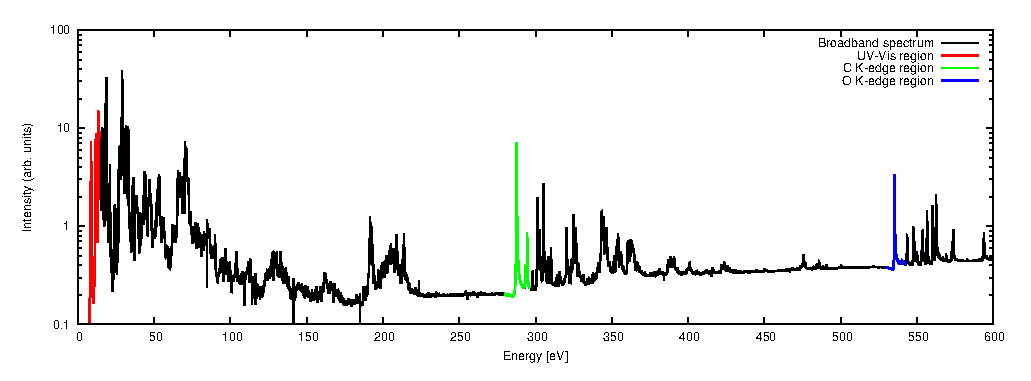
\includegraphics[scale=0.65]{figures/broad.eps}\\
\end{center}
\footnotesize{D. R. Nascimento and A. E. DePrince, {\it JPCL}, {\bf 8}, 2951, (2017)} 
\end{frame}

\begin{frame}{Accelerating convergence using Pad{\'e} approximants}
K-edge absorption spectrum of carbon monoxide
\begin{center}
 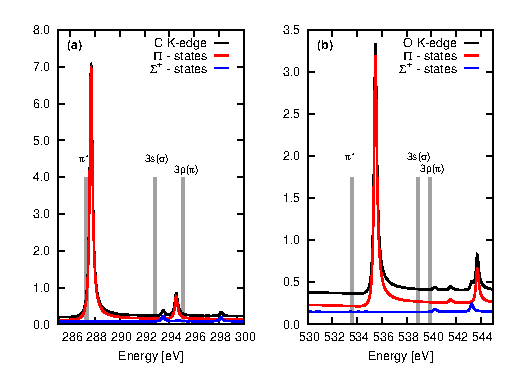
\includegraphics[scale=1.0]{figures/kedge.eps}\\
\end{center}
\footnotesize{D. R. Nascimento and A. E. DePrince, {\it JPCL}, {\bf 8}, 2951, (2017)} 
\end{frame}

\begin{frame}{Exploring new avenues...}
\onslide<1->{
The physical description of the absorption line shape function is that an oscillating external 
electric dipole (the incident field) can induce an oscillating electric dipole in the system 
(the radiating field). 

\begin{equation}
 I(\omega) =  \int_{-\infty}^{\infty}  dt~ e^{-i \omega t} \langle \tilde{ \Psi}_0 | {\color{red}{\bar{\mu}}} e^{i \tilde{H}t} {\color{blue}{\bar{\mu}}}| \Psi_0 \rangle  \nonumber 
\end{equation}
\begin{center}
{\color{blue}{$\bar{\mu} \rightarrow$ incident field}} \\
{\color{red}{$\bar{\mu} \rightarrow$ radiating field}} \\
\end{center}
}
\vspace{10pt}
\onslide<2->{
Thus the oscillator strength for the excited states (within the dipole approximation) can be 
computed as
\begin{block}{}
\begin{equation}
 f(\omega) = \frac{2}{3} \omega \Re\{I(\omega)\} \nonumber
\end{equation}
\end{block}
}
\end{frame}

\begin{frame}{Exploring new avenues...}
\onslide<1->{
But... that's not the whole story! The incident field can also induce an oscillating {\bf magnetic} 
dipole! In fact it induces electromagnetic multipoles.\\
}
\vspace{10pt}
\onslide<2->{
We could instead probe the induced magnetic field: \\
\begin{block}{}
\begin{center}
  {\color{red}{$\bar{\mu} \rightarrow \bar{m}$}}
\end{center}
\end{block}

\begin{equation}
 I(\omega) =  \int_{-\infty}^{\infty}  dt~ e^{-i \omega t} \langle \tilde{ \Psi}_0 | {\color{red}{\bar{m}}} e^{i \tilde{H}t} {\color{blue}{\bar{\mu}}}| \Psi_0 \rangle  \nonumber 
\end{equation}
}
\onslide<3->{
Thus the {\bf rotatory} strength for the excited states (within the dipole approximation) can be 
computed as
\begin{block}{}
\begin{equation}
 R(\omega) = \Im\{I(\omega)\} \nonumber
\end{equation}
\end{block}
}
\end{frame}

\begin{frame}{Exploring new avenues...}
Electronic circular dichroism (ECD) spectroscopy 
\begin{center}
  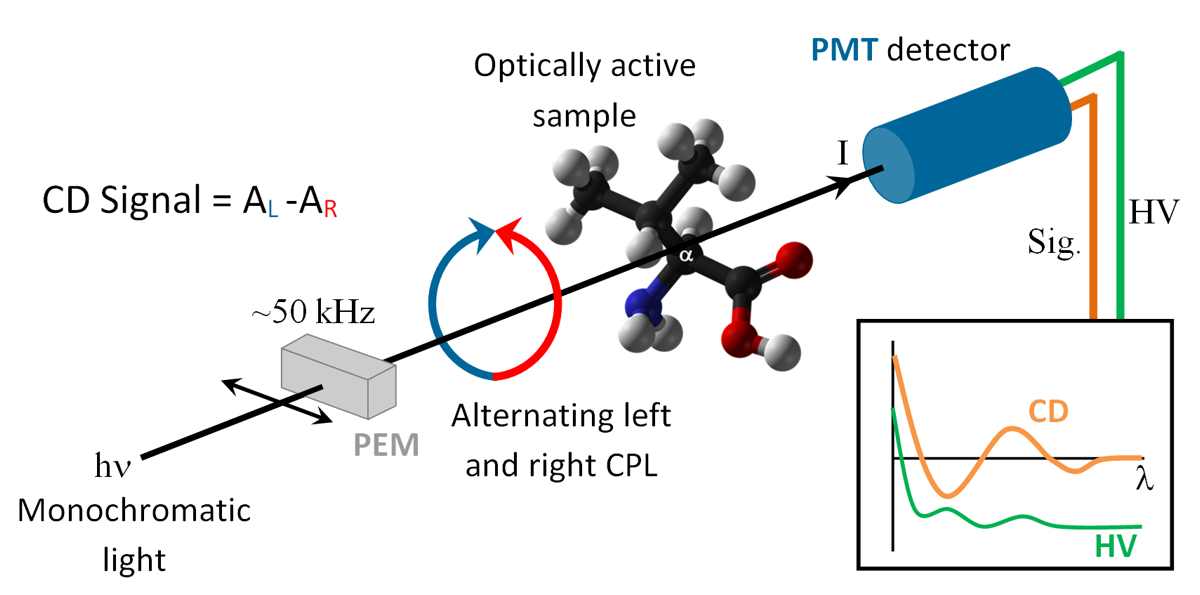
\includegraphics[scale=0.25]{figures/CD.png}
\end{center}
\footnotesize{Credit: © ISA, Centre for Storage Ring Facilities, Aarhus}
\end{frame}

\begin{frame}{Exploring new avenues...}
Electronic circular dichroism (ECD) spectroscopy \hspace{15pt}
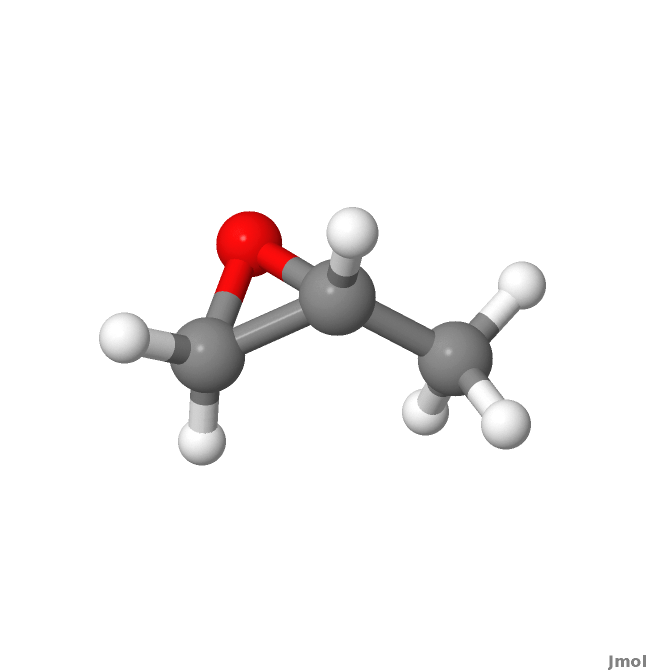
\includegraphics[scale=0.1,trim={1.4in 2.5in 1.4in 1.6in},clip]{figures/methyloxirane.png}
\begin{center}
  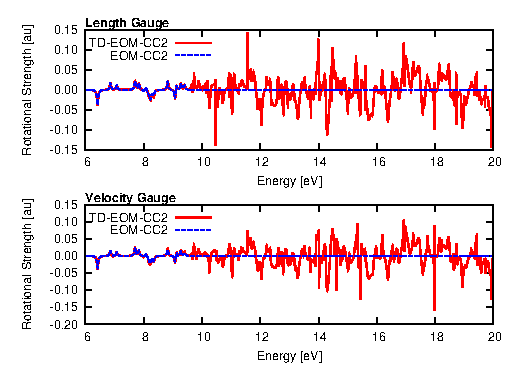
\includegraphics[scale=1.0]{figures/methyloxirane_adz.eps}
\end{center}
\end{frame}

\begin{frame}{Concluding remarks}
\begin{itemize}
\onslide<1->{
 \item Coupled-cluster theory is the ``gold standard'' of quantum chemistry for weakly correlated systems due to its accuracy and robustness. \vspace{5pt}
}
\onslide<2->{
\item Here, we have developed an efficient explicitly time-dependent coupled-cluster framework to simulate broadband absorption spectra of molecular systems. \vspace{5pt}
}
\onslide<3->{
\item We make the use of Pad{\'e} approximants in order to obtain a fully converged spectra without the need to use excessively large simulation times. \vspace{5pt}
}
\onslide<4->{
\item The method can be extended to compute any type of linear absorption spectra. 
}
\end{itemize}
\end{frame}

\begin{frame}{Acknowledgments}
\onslide<1->{
  \begin{figure}
  
\includegraphics[width=0.9in,height=0.9in]{figures/nsf-logo.png} \hspace{15pt}
  
\includegraphics[width=0.9in,height=0.9in]{figures/FSU_seal.png} \hspace{15pt}
  
\includegraphics[width=1.2in,height=0.8in,trim={0 0 0 0.6in},clip]{figures/ACS-PRF.png}
 \end{figure}
}
 \begin{figure}
 \onslide<2->{
   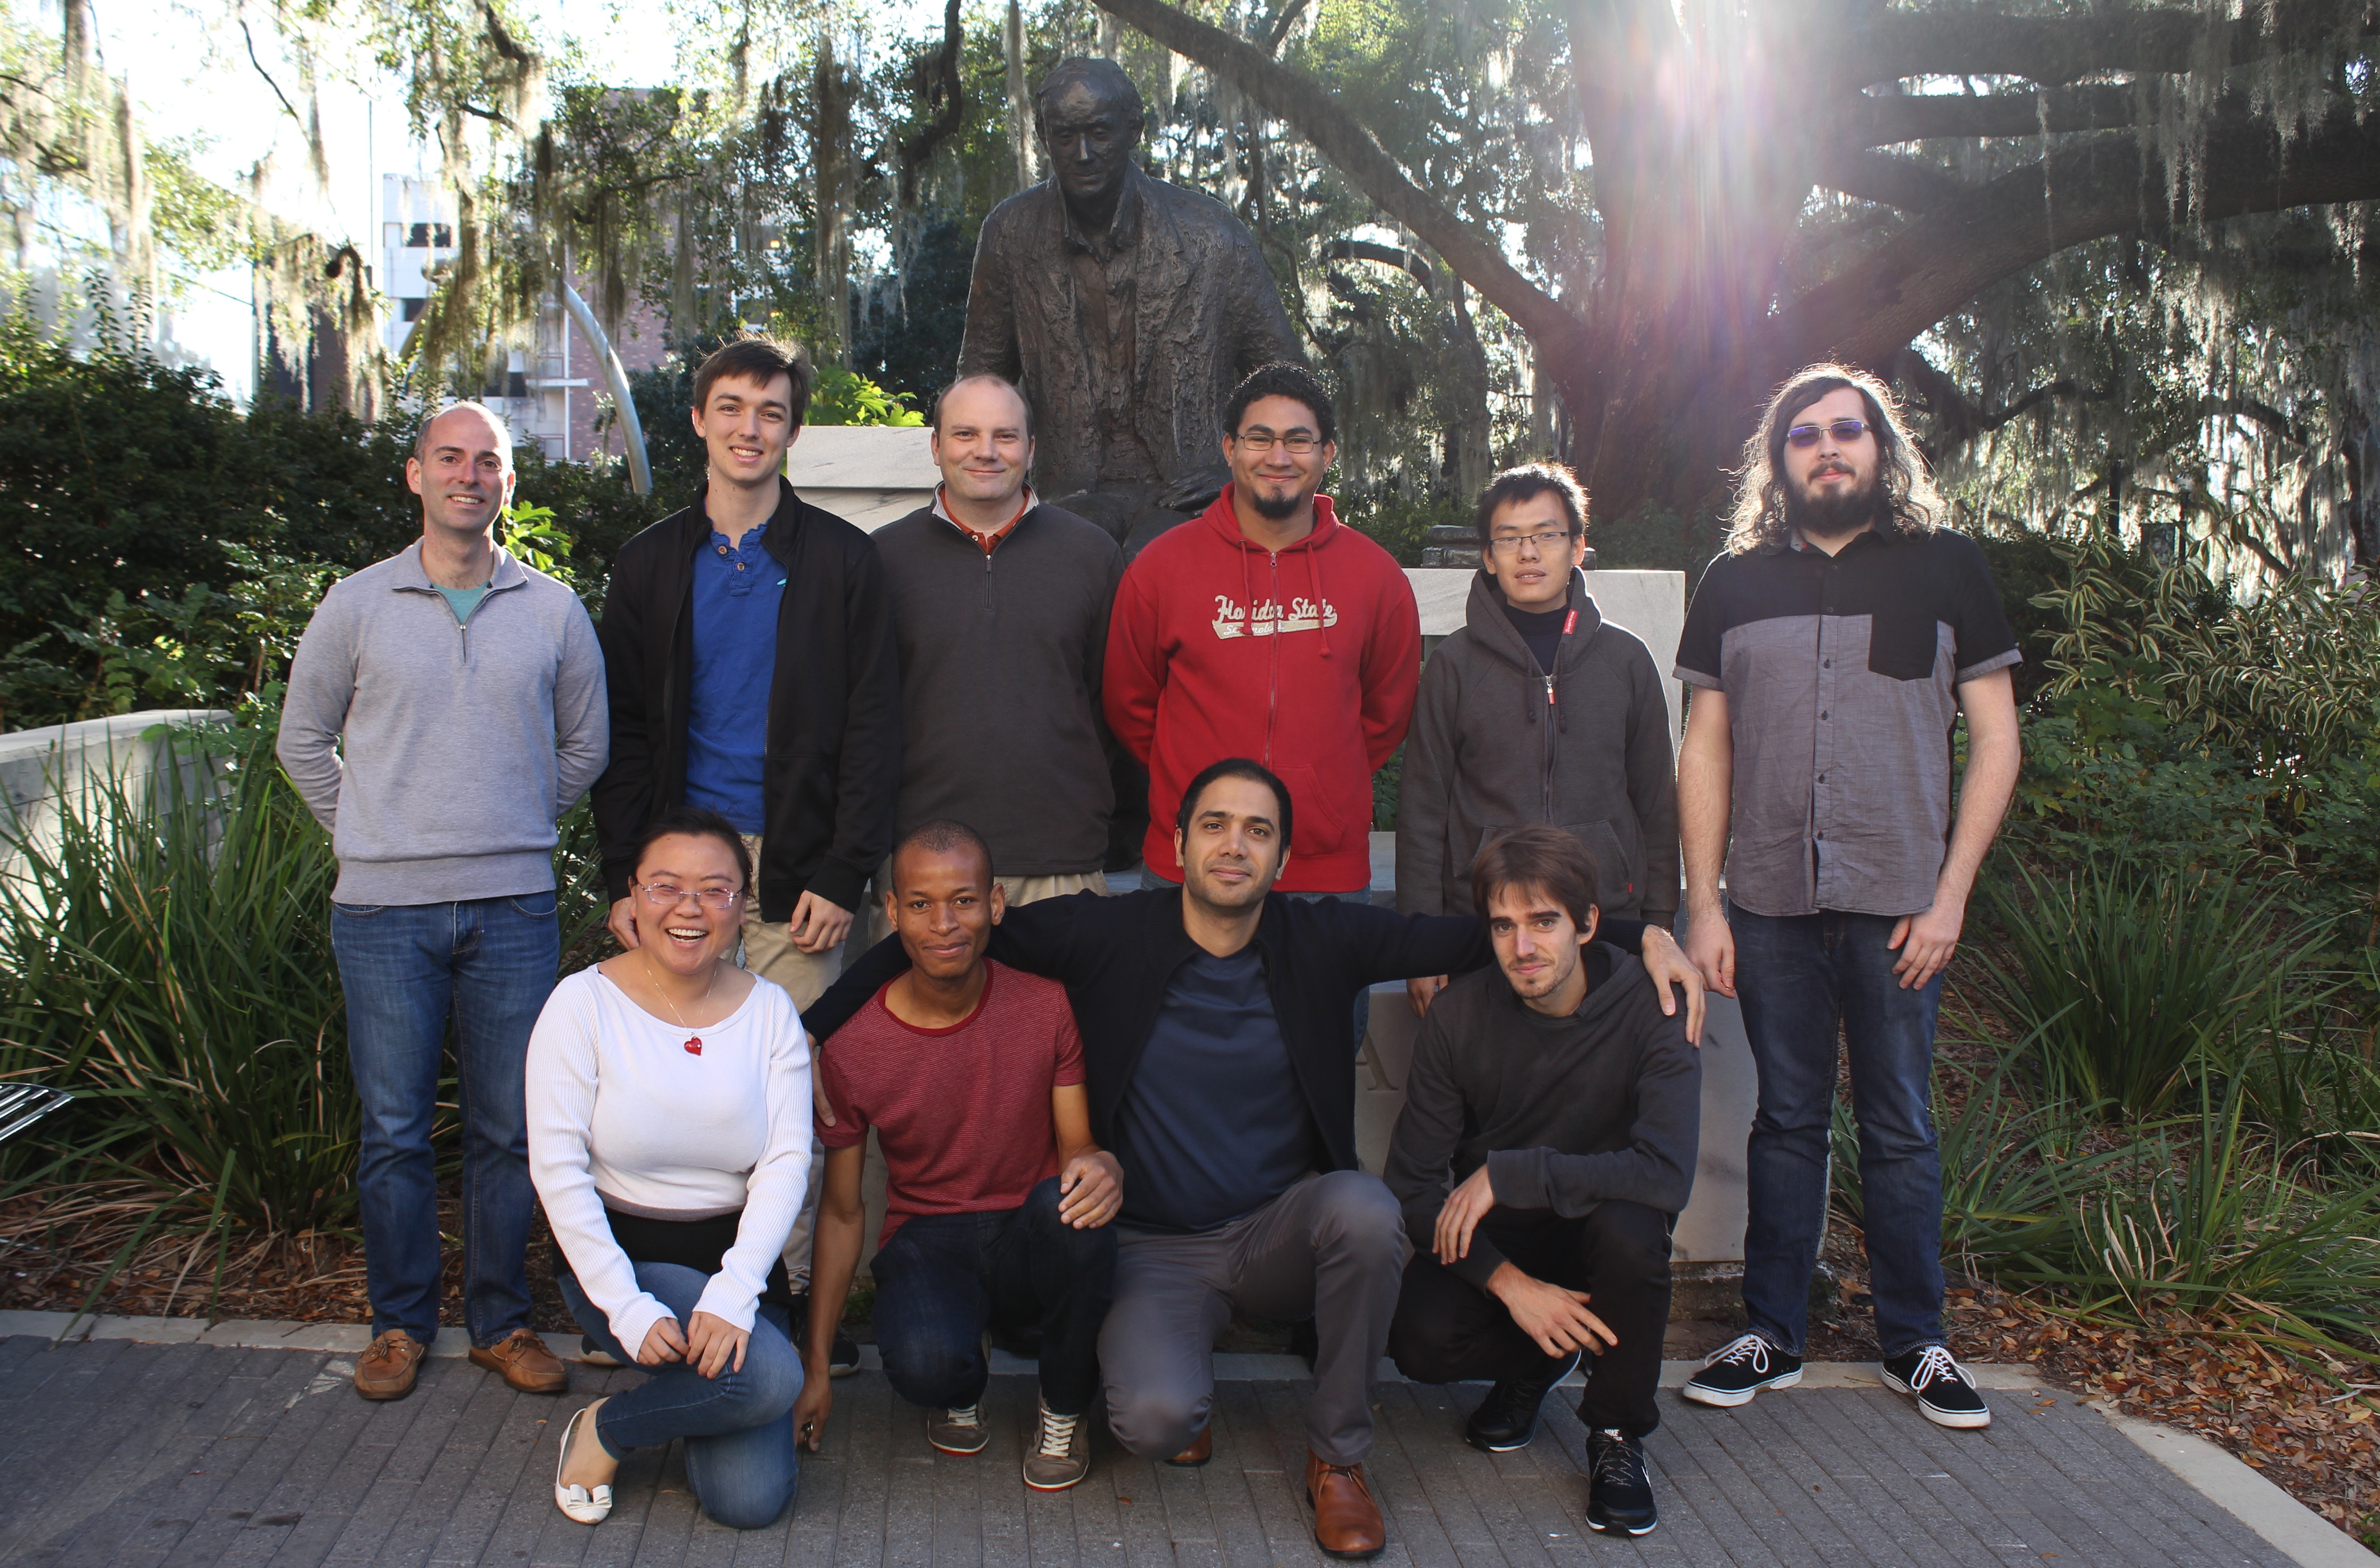
\includegraphics[scale=0.03]{figures/deprince_group_fall_2017.jpg}
 }
 \onslide<3->{  
   \includegraphics[scale=0.033]{figures/Sherrill_group.jpg}
 }  
 \end{figure}
\end{frame}

\begin{frame}
\begin{center}
  \Huge{Thank you!}
\end{center}
\end{frame}


\end{document}
